\documentclass[12pt]{article}
\usepackage{amsfonts}
\usepackage{graphicx}

%%%%%%%%%%%%%%%%%%%%%%%%%%%%%%%%%%%%%%%%%%%%%%%%%%%%%%%%%%%%%%%%
%
% dimensions choisies par l'utilisateur (bricolage personnel)

\newdimen\decalage

\paperheight=29.7 true cm \paperwidth=21 true cm
\textheight=25.7 true cm \textwidth=17 true cm
\decalage=0 true cm

% déduction de \topmargin,
% \evensidemargin et \oddsidemargin

\oddsidemargin=\paperwidth
\advance\oddsidemargin by -\textwidth
\divide\oddsidemargin by 2
\advance\oddsidemargin by -1 in
\evensidemargin=\oddsidemargin
\advance\oddsidemargin by \decalage 
\advance\evensidemargin by -\decalage

\topmargin=\paperheight
\advance\topmargin by -\headheight
\advance\topmargin by -\headsep
\advance\topmargin by -\textheight
\advance\topmargin by -\footskip
\divide\topmargin by 2
\advance\topmargin by -1 in

%
%%%%%%%%%%%%%%%%%%%%%%%%%%%%%%%%%%%%%%%%%%%%%%%%%%%%%%%%%%%%%%%%

\begin{document}

\title{Compte rendu du TP3 - Fourier}
\author{Louis Allain}
\maketitle

\section{Séries de Fourier}

Réponses aux question :
\begin{enumerate}
	\item 
		La période du signal est $T_0 = \frac{2}{\pi}$. \\
		La pulsation du signal $\omega_0 = \frac{2\pi}{T} = 1$ où $T = 2\pi$. \\
		La fréquence du signal $f_0 = \frac{1}{T_0} = \frac{1}{2\pi}$. \\
		
	\item
		On doit prendre $f_s$, la fréquence d'échantillonnage tel que 
$f_s \geq 2.Nf_0$ où $Nf_0$ est la fréquence la plus grande de la dernière harmonique que l'on choisi. \\
		$$
			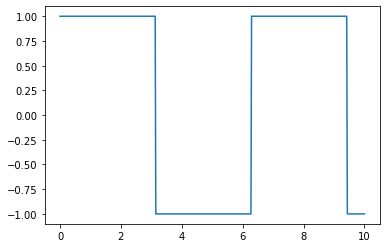
\includegraphics[width=0.8\textwidth]{q2_dessin_signal_carre.PNG}
		$$
		
	\item
	Réécriture de s à partir de la composition de s en série de Fourier :\\\\
		$s(t) = \frac{4}{\pi} \sin(2\pi(f_0)t) + \frac{4}{3\pi} \sin(2\pi(3f_0)t) + \frac{4}{5\pi} \sin(2\pi(5f_0)t) + ... + \frac{4}{N\pi} \sin(2\pi(Nf_0)t)$\\\\
		Les conditions que s doit respecter sont les conditions de Dirichlet. La première condition est que s doit être continue par morceaux. La seconde est que s doit être monotone par morceaux. Et enfin, la troisième condition est que s doit être partout intégrable.
		
	\item
		A faire.
		
	\item
		Les equations générales permettant de calculer les coeffecients de Fourier : $a_k$ et $b_k$: \\\\
		$a_k = \frac{2}{T}\int_{\frac{-T}{2}}^{\frac{T}{2}}s(t)\cos(nt\frac{2\pi}{T})$\\\\
		$b_k = \frac{2}{T}\int_{\frac{-T}{2}}^{\frac{T}{2}}s(t)\sin(nt\frac{2\pi}{T})$.\\\\
	
	\item 
		Pour le signal s, \\\\
		$a_0 = 0$,\\
		$a_k = 0$,\\
		$b_k = \frac{4}{k\pi}$ pour k impair,\\
		$b_k = 0$ pour k impair.
		
	\item
		Calcul d'un terme de la série de Fourir en Python :
		\begin{verbatim}
		terme = (2*(1-(-1)**k)*np.sin(k*x))/(k*(np.pi));
		\end{verbatim}
		
	\item 
		Programme Python serieFourier (d'après le cours) :
		\begin{verbatim}
			def serieFourier (ordre, N) :
					 
			R = np.zeros(N)  
			t = np.linspace(0,((N-1)/N)*2*(np.pi),N)     
			
			for i in range(N):
					x = t[i]           
					y = 0 
					
					for k in range(1,ordre+1):             
							terme = (2*(1-(-1)**k)*np.sin(k*x))/(k*(np.pi))             
							y = y + terme
							
					R[i]=y   
			return R 
		\end{verbatim}
		
	\item
		Plus N se rapproche de l'ordre plus on retrouve le signal carré. Mais la convergence vers ce signal est lente et de l'ordre de $\frac{1}{k}$.
		
	\item 
		Affichage de manière superposée les décompositions de s :
		\begin{verbatim}
			for i in range(1, 100, 3):
				plt.plot(serieFourier(i, 100))
		\end{verbatim}
		Et voici le résultat graphique :\\
		$$
			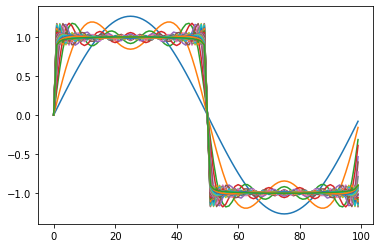
\includegraphics[width=0.8\textwidth]{q10_decomposition.PNG}
		$$
		
	\item 
		On observe le phénomène de Gibbs, il semble que c'est un effet de dépassement du max de s(t).
		
\end{enumerate}

\section{Transformée de Fourier}

Réponses aux question :
\begin{enumerate}
	\item 
		Sinuisoïde de fréquence 16 Hz :
		$$
			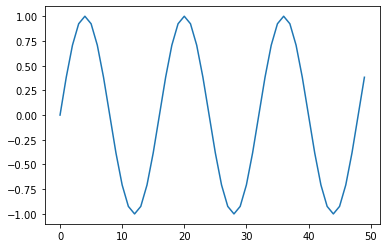
\includegraphics[width=0.8\textwidth]{q2_1.png}
		$$
		
	\item
		 On souhaite changer d’espace de représentation en utilisant la transformée de Fourier du signal s.
	
	\item
		Calcul du spectre :
		\begin{verbatim}
			TFD = fft(echantillons) # spectre
			A = np.absolute(TFD/N) # amplitude
			An = A/A.max() # ampmlitude normalisée
			P = np.angle(TFD/N) # phase normalisée
		\end{verbatim}
	
	\item
		Affichage du spectre :
		$$
			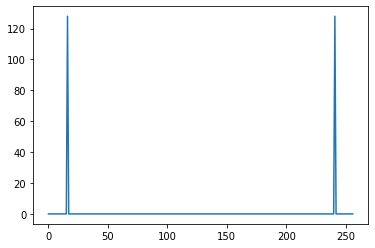
\includegraphics[width=0.8\textwidth]{q2_4.png}
		$$
		On observe dans le spectre une seconde raie. Cela est du au fait que ce signal est périodique.
	\item
		On observe un élargissement de la base des raies du spectre. Cela est du à la durée fini de l'échantillonnage.
		En effet, si la durée d'échantillonnage était infinie, les raies seraient de largeur 0.
		$$
			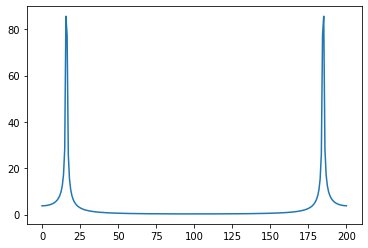
\includegraphics[width=0.8\textwidth]{q2_5.png}
		$$
	\item
		$$
			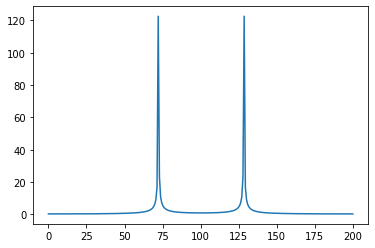
\includegraphics[width=0.8\textwidth]{q2_6.png}
		$$
		On peut observer une raie à k=128 mais également une autre raie à une fréquence inférieure. 
		Cela est du à un effet de repliement. En effet, si l'on ne respecte pas le théorême de Shannon-Nyquist (fs >> fmax), le spectre se replie sur lui même.
		
	\item
		\begin{verbatim}
			Créer le signal numérique suivant :
			x = 3*math.cos(50*pi*t) + 10*math.sin(300*pi*t) - math.sin(100*pi*t)
		\end{verbatim}
\end{enumerate}
\end{document}